\documentclass[12pt]{article}
\usepackage{amsmath,amssymb,amsthm}
\usepackage{fullpage}
\usepackage{graphicx}
\usepackage{hyperref}
\newtheorem{thm}{Theorem}[section]

\theoremstyle{definition}
\newtheorem{defn}{Definition}[section]
\newcommand{\floor}[1]{\left\lfloor #1 \right\rfloor}
\newcommand{\ceil}[1]{\left\lceil #1 \right\rceil}
\begin{document}
\title{A strategy for lower-bounding clique detection, combining
Shannon's counting argument with clique covers of random hypergraphs}

\author{Josh Burdick ({\tt josh.t.burdick@gmail.com})}
\maketitle
\begin{abstract}
Shannon's function-counting argument
\cite{shannon_synthesis_1949} showed that some Boolean functions have
exponential circuit complexity, but doesn't provide a specific example
of such a hard-to-compute function. A simple modification of that argument
shows that detecting a randomly-chosen subset of the $k$-vertex cliques in an
$n$-vertex graph requires, on average, $\Omega(n^{k/2})$ NAND gates.
This doesn't directly bound the complexity of detecting {\em all} of the cliques.
However, we can view a random subset of cliques as a randomly-chosen
$k$-regular hypergraph on $n$ vertices.
If we can cover such a hypergraph with large enough cliques,
and we could detect cliques with few enough gates, we would contradict
the average-case counting bound described above.
Probablistic graph theory arguments
\cite{bollobas1976cliques} similar to \cite{bollobas1993clique}
allow bounding the number of cliques needed to
cover a random hypergraph.
This provides a strategy for lower-bounding clique detection.
We suggest several possible ways of covering hypergraphs with cliques,
and numerically evaluate this bound for small graphs, finding that
it barely gives a positive bound.
\end{abstract}

I am writing this up on the assumption that the modification
to Shannon's counting argument (section \ref{countingBound})
is not new. It doesn't seem to give a bound larger than 1.
I'm hopeful that it is correct and/or that it has useful bits,
or that someone can point me
to similar lower-bound attempts; or, if it's wrong, that 
someone can point out the flaw(s).

\newpage

\tableofcontents

\section{A counting bound} \label{countingBound}

The first argument is basically a function-counting argument.

\subsection{Background: lower bounds from function counting}

It's long been known that computing {\em some} function of a bit-string
requires exponentially large circuits \cite{shannon_synthesis_1949}.
If there are $m$ inputs to a circuit,
then there are $2^{2^m}$ possible functions from the $m$-input bitstring to
a one-bit output. Each of these functions, being different, must have a
different circuit.

If we assume the circuit is made of NAND gates, and has $g$ gates, then the
circuit could have at most $gm$ wires from inputs to gates, and ${g \choose 2}$
wires from gates to gates. We can view the possible circuits as a bitmask,
containing a 1 everywhere a gate is connected to an input (or another gate),
and 0 everywhere else.

\begin{thm}
\label{boundFromCounting}
Consider functions from $m$ bits to one bit of output.
This means that, with $g$ gates, we can represent at most
$2^{gm + {g \choose 2}}$ different boolean functions (with $m$ bits of input,
and one bit of output).
\end{thm}
\begin{proof}

The number of possible wires which are there, or not, is $gm + {g \choose 2}$,
which bounds how many possible circuits there are.
Some of these circuits compute the same function.
However, there can't be any more than this many circuits with this many wires.
\end{proof}

This means that if we have a large set of functions, and we know the size of
the set of functions, then we know that at least {\em one} of them requires
a large number of gates. (Knowing {\em which} function requires a lot, or many,
gates is still an issue).

Consider functions from $m$ bits to one bit of output.
Let $g$ be the number of gates, and $w$ be the number of wires.
Solving for the number of gates:

\begin{eqnarray*}
w & = & mg + {g \choose 2} \\
  & = & mg + g(g-1)/2 \\
  & = & mg + (g^2 - g) / 2 \\
  & = & 0.5g^2 + (m-0.5)g \\
0 & = & 0.5g^2 + (m-0.5)g - w \\
\end{eqnarray*}

We solve the quadratic formula (writing $b = m-0.5$ for simplicity), keeping
only the non-imaginary root.

\begin{eqnarray*}
g & = & -b \pm \sqrt{ b^2 + 2w} \\
  & = & {\sqrt {2w + b^2}} - b \\
\end{eqnarray*}

Thus, given a set of functions, we know that at least one of them requires
some number of gates.

\subsection{Bounding the average number of gates}

We can also count the total number of functions from $m$ input bits to one
output bit, using up to $g$ NAND gates, as

\begin{eqnarray*}
\sum_{i=0}^{g-1} 2^{m+i} & = & 2^{m+g} - 2^m
\end{eqnarray*}

If we're counting circuits with up to $g$ gates, then some of the circuits
have fewer than $g$ gates. This somewhat complicates the book-keeping.
However, {\em most} of the
circuits have $g$ gates. (Indeed, well over half, since each additional
gate adds many potential wires). Because of this, I think that the
average case bound is just one fewer gates than the worst-case bound.


\subsection{Counting CLIQUE-like functions}

We now consider NAND gate circuits (with any fan-in) which find $k$-cliques in $n$-vertex
graphs.

We consider the set of ``buggy'' 6-clique finders. 
Maybe the circuit correctly
finds all the cliques. Or maybe it finds all of the cliques except $K_{1..6}$,
or it misses half the cliques, or finds none (and always outputs 0), or maybe
it only successfully finds $K_{1,3,4,5,7,8}$, or whatever. More formally
(and generally),
we define a set of functions ({\em not} circuits):

\begin{defn}
\label{BUGGY-k-CLIQUE}
BUGGY-$k$-CLIQUE$(n)$ is the set of functions which recognize any set
of $K_k$s. That is, for each set $A$ of $K_k$s, BUGGY-$k$-CLIQUE$(n)$
contains a function which is 1 if the input contains any $K_6 \in A$,
and 0 otherwise.
\end{defn}

This clearly includes HAS-$k$-CLIQUE (which finds all the cliques).

These functions are all distinct. If $f_1,f_2\in $BUGGY-$k$-CLIQUE$(n)$,
then there's some $K_k$ such that if $y$ is the graph with {\em only}
1's in that $K_k$ (and 0's elsewhere), $f_1(y) = 0$ and $f_2(y) = 1$.

Of course, many of these functions are quite similar (e.g. all but one of them
output a 1 when you feed in all 1's). However, they're all slightly different.

\begin{thm}
\label{buggyDistinct}
BUGGY-$k$-CLIQUE$(n)$ contains $2^{n \choose k}$ distinct functions.
\end{thm}
\begin{proof}
That's how many subsets of the $K_k$s there are.
\end{proof}

Although $2^{n \choose k}$ is a fairly large number,
it's still comfortably less than $2^{2^{n \choose 2}}$, the number of boolean
functions on the ${n \choose 2}$ input wires (one per edge).

\subsubsection{But {\em which} function requires many gates?}

So, there are $2^{n \choose k}$ different functions. 
How many NAND gates do these take?
(We onsider NAND gate circuits (with any fan-in) which find $k$-cliques in $n$-vertex
graphs, as a circuit with $n \choose 2$ inputs)

Applying Theorem
\ref{boundFromCounting}, we know that at least one of the circuits requires
${\sqrt {2 {n \choose {k/2}} + b^2}} - b = \Omega(n^{k/2})$ 
NAND gates (where $b = {k \choose 2} - 0.5$).

Why doesn't this bound HAS-$k$-CLIQUE?
Because we don't know that the circuit which finds {\em all} of the
$K_k$s, is one of these larger circuits. As far as what I've
shown thus far goes, it could be harder to find some weird subset of the $K_k$s.

Indeed, as far as what I've formally shown goes, the problem which needs
the most NAND gates could be finding a single $K_k$! That's easily ruled out
(because that only needs one NAND gate, plus the output gate).

\subsection{Which sets of cliques are hard to find?}

The hardness of these functions depends
on how the cliques they find are laid out.
For instance, here are two sets of 20 triangles (``$K_3$s''),
arranged in different ways. Although we only show 20 triangles here,
we can imagine similarly-structured graphs with more triangles.

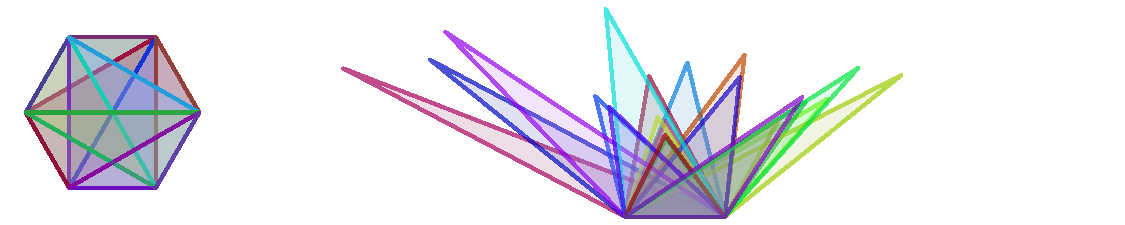
\includegraphics[width=0.9\textwidth]{R/tri1.pdf}



Triangles can be detected using matrix multiplication \cite{itai_finding_1977},
and there are fast algorithms known for matrix multiplication
\cite{strassen_gaussian_1969}
\cite{williams_multiplying_2012}, so
the triangles on the left can be detected
using fewer than one NAND gate per triangle (for large enough input graphs).
\footnote{For smaller graphs, such as this with six vertices,
it appears that 21 NAND gates are required
\cite{burdick_triangles_6_vertex},
although this proof hasn't been published or rigorously checked.}

On the other hand, if the triangles overlap less (as on the right),
then to detect all of the triangles, we will definitely need at least one
gate per triangle.
To see this, note that if we feed in a 0 to the input for one
of the edges unique to some triangle, then any gate connected to
that edge will only output a 1. We can repeat this for each of the
triangles, constructing a series of strictly smaller circuits
(this is essentially what I think is called
the ``method of restrictions'' FIXME CITE).

It seems intuitive that, in some sense, finding more cliques should
be harder.
Indeed, since we're using NAND gates, we know that finding any non-empty
subset of cliques is strictly harder than finding {\em some} other 
smaller set of cliques (namely, the set you get after feeding in 0's to
all the edges connected to some vertex).
Unfortunately, this doesn't help much
in the case of CLIQUE.  If we have a circuit which
finds 6-cliques on 100 vertices, and feed in 0's to all edges connected to
one vertex, we
end up with a strictly smaller circuit which finds 6-cliques on
99 vertices! We still haven't connected the complexity of CLIQUE with
the complexity of all those ``buggy'' circuits which find exactly half
the cliques.

\subsection{Counting slightly larger sets of functions}

We can also construct somewhat larger sets of functions. For instance,
suppose that, rather than detecting or ignoring each clique, we assign
to each edge either 1, 0, or X, with this interpretation:

\begin{itemize}

\item 1: ``If any of these cliques is present, then output 1...''

\item 0: ``...unless one of these cliques is present, in which case output 0.''

\item X: ``(Ignore whether this clique is present).''

\end{itemize}

There are $3^{n \choose k}$ such strings. However, those consisting only of
0's and X's always output 0, and so are indistinguishable, so there are
only $3^{n \choose k} - 2^{n \choose k}$ distinct functions.

The lower bound on the average hardness of computing these functions is
slightly higher. However, this doesn't seem to help that much.

Note that distinguishing the functions requires that we be able to have at
least two distinct cliques either be present or absent. With two cliques,
we can do this by feeding in 1's to any edges shared by the cliques, and
then feed in 0's or 1's to the remaining edges:

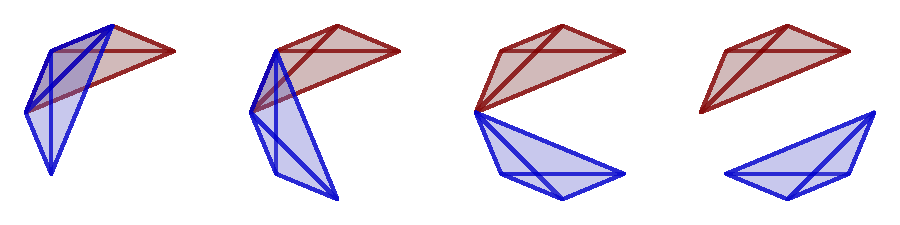
\includegraphics[width=0.7\textwidth]{R/overlapping.pdf}

However, it seems hard to push this to arbitrary functions of ``which cliques are
present'', because they start to overlap.

\section{Bounds based on covering hypergraphs with cliques}

Suppose we consider all $2^{n \choose k}$ functions which find some subset
of $k$-cliques in an $n$-vertex graph, and for each, find the circuit with
the fewest NAND gates which computes it. If we add up the total number of
gates in all of these circuits,
it's a lot. Since they're all distinct functions, the
function-counting bound gives a lower-bound on
the total number of gates used (as from the
above, we know how many functions from $m$ inputs to one output
we can implement using $g$ NAND gates).

Note that, for a given set of $k$-cliques $S$, if $S = A \cup B$, and we
have circuits to find the $k$-cliques in $A$ and $B$, then by ORing them
together, we obtain a circuit for $S$. (If we use NAND gates, we
save a gate. Given circuits for $A$ and $B$, to construct a circuit
for $A \cup B$, we can disconnect the wires from $B$'s last gate, and
connect them to $A$'s last gate. $A$'s output now computes $A \cup B$,
and $B$'s last gate is no longer needed). (FIXME add a figure?)

Suppose we had small circuits for detecting all of the $k$-cliques
in an $r$-vertex graph, for $k \le r \le n$.
Then, one way to generate a circuit which finds an arbitrary subset
of $k$-cliques would be to decompose it into a set of
cliques (of size between $k$ and $n$), and OR them all together.

Suppose we do this, for {\em all} of the $2^{n \choose k}$ possible subsets of
$k$-cliques. We then add up the total number of clique detectors of each
size that we've used, and total up how many NAND gates are in each of these.
We had better have used at least as many NAND gates as the Shannon counting
bound says we needed, to implement all of those functions.

To be more concrete: suppose we
devise a way of covering all the $k$-cliques in an $n$-vertex
graph. Instead of counting across all possible sets of cliques, we will
consider the average, for a set of cliques chosen uniformly at random.
Let $k$ be the size of cliques we're bounding the complexity of finding,
choose some covering strategy, and let:

\begin{itemize}

\item $A_{ij}$ = the average number of $j$-vertex hypercliques (``$K^j_k$''s)
in an $i$-vertex graph

\item $x_{j}$ = the number of gates needed to find $k$-cliques on $j$ vertices

\item $b_{i}$ = the Shannon bound on the number of
gates needed (on average) to find any set of $k$-cliques on $i$ vertices

\end{itemize}

We have

\[
Ax \ge b
\]

This gives a lower bound on $x$. The bound depends
crucially on how efficiently
we can cover the hyperedges with hypercliques -- in order for $x$ to
be large, we need the entries of $A$ to be as small as we can manage.
(Presumably, we need as many of
the cliques as possible to be large, and to not overlap much).
We can choose as many different rows of this as we like.
However,
adjacent rows will presumably give very similar bounds, so it may be
simpler to only use a subset of rows.
It's not obvious that this even bounds $x$ to be positive.

\subsection{Anecdotal rephrasing}

(I include the following hypothetical anecdotal explanation,
partly because I think it's slightly funny, but also because I think it may
provide at least some intuition).

In some alternate reality, it is the dawn of the era of 
TTL integrated circuits.
Yoyodyne Corporation has developed a line of integrated circuits to detect
any possible set of $K_4$s in a graph with nine vertices.
These chips, the 74LSC series,
are available in a convenient 40-pin DIP package, and are
fabulously successful. (I have no idea why there would be huge demand for
these, but let's say that there is). The only problem is that Yoyodyne's 
chip factories are having trouble producing enough chips.

Management contemplates how to re-envision productivity and enable
synergy. (They are, after all, producing $2^{9 \choose 4} = 2^{126}$
different sorts of chips).
They decide that they need to stop producing so many kinds of chips.
After great deliberation, they decide to cut production to {\em just} the
chips which find all possible
$K_4$'s on graphs with between four and nine vertices (namely, the 74LSC4
through 74LSC9). In order to meet the bizarre but humongous
demand for finding arbitrary sets of $K_4$s, they will develop a
line of tiny circuit boards,
each containing several clique detectors, ORed together.

There is still the problem of designing these circuit boards. However,
they only have to do this once for each possible set of $K_4$s. They hire
a large team of software engineers and graph theorists. By renting
many years of CPU time from AltaVista and MySpace, they are able to design the
optimal circuit boards.

Note that, originally, Yoyodyne was using some number of NAND gates to
cover all the $2^{9 \choose 4} = 2^{126}$ possible sets of $K_4$s.
The Shannon counting
argument gives a lower bound on how many NAND gates were used in all of
these chips. (Specifically, it says that at least four NAND gates
were used for at least one graph, since $36+37+38+39 = 150 \ge 126$).

After the redesign, if 
we count up the number of 74LSC4 through 74LSC9 gates which were used,
and consider the number of NAND gates in each
of these, the total had better {\em also} be larger than the bound from
the Shannon counting argument.

\subsection{How do we cover the graphs?}

Thus, we are faced with the problem of covering all possible $2^{n \choose k}$
sets of cliques with a small number of large cliques.
We can think of a set of possible $k$-cliques as
a $k$-regular hypergraph on $n$ vertices. Clique cover (for non-hypergraphs)
is a well-known NP-complete problems \cite{karp1972reducibility}.
In our case, we are covering hypergraphs with hypercliques. Also,
we aren't concerned with the complexity of finding the
covering. However, we do need to know how many hypercliques of various sizes are
needed.

Here, we describe covering strategies of increasing simplicity. We then
try to apply the simplest strategy in section \ref{oneCliqueSize}.

(FIXME It's tempting to omit the ``hyper'' from
``hypergraph'', ``hyperedge'', etc. However, it might be good to include,
to distinguish from the original clique-detecting problem).

\subsection{Using the set-cover greedy algorithm}

Suppose we're given a $k$-regular (hyper)graph, and are trying to cover it
with a small number of (hyper)cliques. This is reminiscent of the
set cover problem, in which we are trying to cover some elements with
a small number of sets.  There is a greedy
strategy for set-cover, which consists
of simply picking the set which covers the most elements, removing those
elements, and repeating \cite{chvatal1979greedy}.
This has a guaranteed approximation ratio.

This suggests the following strategy. Pick the largest clique, remove it, and
repeat. If we do this, then each time we remove a clique, we know exactly
how much the density of the graph is reduced. If we know that a
sufficiently-dense graph has a fairly large clique, then we should be able
to bound how many cliques of each size we decomposed the original graph into.

It's known that if a conventional graph (that is, a graph
in which each edge has two vertices, or ``2-regular graph'')
has many edges, then it must contain a clique of a certain size.
Finding the densest graphs which lack some size of clique was an
early problem in extremal graph theory. Since these maximally dense graphs
(the Tur\'an graphs) have a known structure, the size of the clique is
known precisely \cite{turan1941external}.

Generalizing this to hypergraphs seems like a natural question.
Based on the neatness of the solution for 2-regular graphs,
we might guess that, if we know that a $k$-regular hypergraph is dense,
then it must contain a fairly large clique, with a closed-form size.
Unfortunately, for hypergraphs, there doesn't seem to be as neat
an answer as there was for 2-regular graphs. 
If we choose a $k$-regular hypergraph uniformly at random,
``most'' of the subsets of cliques will have about half the
possible number of hyperedges. But at that density,
the known
bounds can't guarantee that there will be many cliques for us to cover.
There is a large gap in the density of graph having some size
of clique
\cite{keevash2011hypergraph}. We omit the details of this, but
roughly speaking,
the largest graph in a random hypergraph doesn't seem likely to be
guaranteed to be ``very large''.

This strategy may be workable, but seems complicated, and we don't pursue
it further here.
However, it is funny to consider that if we {\em could} find a
bound for $k$-regular graphs with $k \ge 3$
(for which Erd\"os offered \$1,000 \cite{keevash2011hypergraph}),
{\em and} it turned
out that the bound implied that sufficiently dense hypergraphs always had
``large'' hypercliques, then we also {\em might} have a
lower bound on CLIQUE.

\subsection{Non-constructively covering random hypergraphs}

The lack of large hypergraph Tur\'an bounds was initially discouraging.
However, that problem (which possibly founded extremal graph theory?) is
``extreme'' in the sense that it looks for the densest graph which lacks
a clique. It pays little attention to the average case.

Also, Keevah's review notes that when a hypergraph is dense enough to
definitely contain some subgraph, it's apt to contain that subgraph
``all over the place'' \cite{keevash2011hypergraph}, a phenomenon
known as ``supersaturation''.  This seems similar to what's
described in \cite{bollobas1976cliques}, which suggests that most of
the cliques in a random graph have a somewhat narrow range of sizes.
This suggests that even if there isn't definitely a huge hyperclique,
there may at least be many smallish hypercliques.

Thus, we try to use random graph theory to upper-bound how many
$r$-vertex clique detecters (on average, or total). We will actually
try to use all of the maximal cliques in a graph (that is, all of the
cliques which are not part of a larger clique). This is presumably
somewhat inefficient.
For instance, in this toy example in which we're covering edges
(``$K_2$''s), there
are four maximal $K_3$s, but we could cover the edges with
only three $K_3$s.
Presumably similar things happen with hypergraphs.

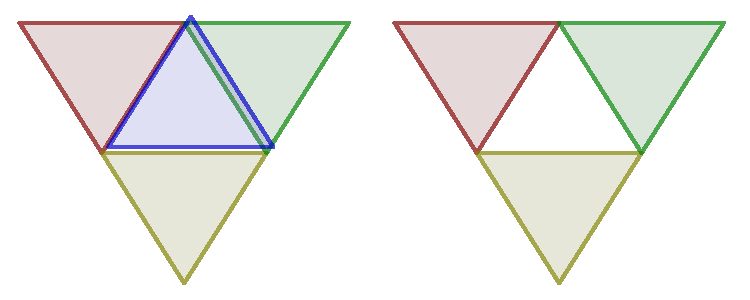
\includegraphics[width=0.5\textwidth]{R/maximal.pdf}

One model of random graphs
includes each edge with some fixed probability. Using this model,
\cite{bollobas1976cliques}
counts the expected number of hypercliques in a hypergraph. Assuming all
edges are chosen i.i.d. (in our case, with probability 1/2),
there are ${n \choose r}$ possible $r$-vertex hypergraphs which might
occur. Each of these is present if ${r \choose k}$ edges are present; as it
were, if that many coins all come up heads. Then the total number of times
we expect this to happen, as noted in \cite{bollobas1976cliques}, is

\[
{n \choose r} \cdot 2^{-{r \choose k}}
\]

Note that these could very well overlap. However, this isn't a problem for
us in terms of correctness. If we cover some clique
with more than one
clique detector, we're
ORing all the detectors together anyway. (This may be wasteful, and it's
possible that we could manage better by only using some of the inputs to
some clique detectors. For now, we ignore this possibility.)

\subsubsection{How often do big hypercliques cover smaller ones?}

The above bound counts hypercliques of different sizes, but has much overlap.
Every time the graph contains a 15-vertex hyperclique, that includes
15 14-vertex hypercliques, ${15 \choose 13}$ 13-vertex hypercliques,
tons of 8-vertex hypercliques, etc. We want to
cover this with one 15-vertex clique detector.

Instead, we consider the odds of a given $r$-vertex hyperclique $A$
being completely
covered by an $r+1$-vertex hyperclique. This requires, for a given vertex
$v$, that all ${r \choose {k-1}}$ edges (consisting of $v$ plus $k-1$ vertices
of $A$) be present. $v$ could be any of $n - r$ vertices; if at least one
 of those
``completes'' $A$, then $A$ is covered. We're interested in counting the
probability that this {\em doesn't} happen (as that's the number of smaller
hypercliques we need to cover). That fraction is

\[
\Big[1 - 2^{-{r \choose {k-1}}}\Big]^{n - r}
\]


\subsubsection{Checking the clique count estimates}

These predictions made me slightly wary, as the events they were counting
aren't independent.
To check them (at least for {\em small} graphs), we used brute force.
Suppose $n, k$ are small enough that we can 
store the adjacency matrix of a $k$-regular graph as a bitvector, and precompute
all possible hypercliques
(with up to $n$ vertices) as bitvectors. Then we can easily generate
random graphs (as bitvectors), count the cliques, and compare that to the graph
density. (Or possibly use the greedy set-cover strategy, and see how
many cliques are need, for random graphs).
We can then compare statistics about the cliques with predictions,
based on \cite{bollobas1976cliques}.
(In the following graphs, the dotted line is the prediction, and
the solid line is the average of samples).

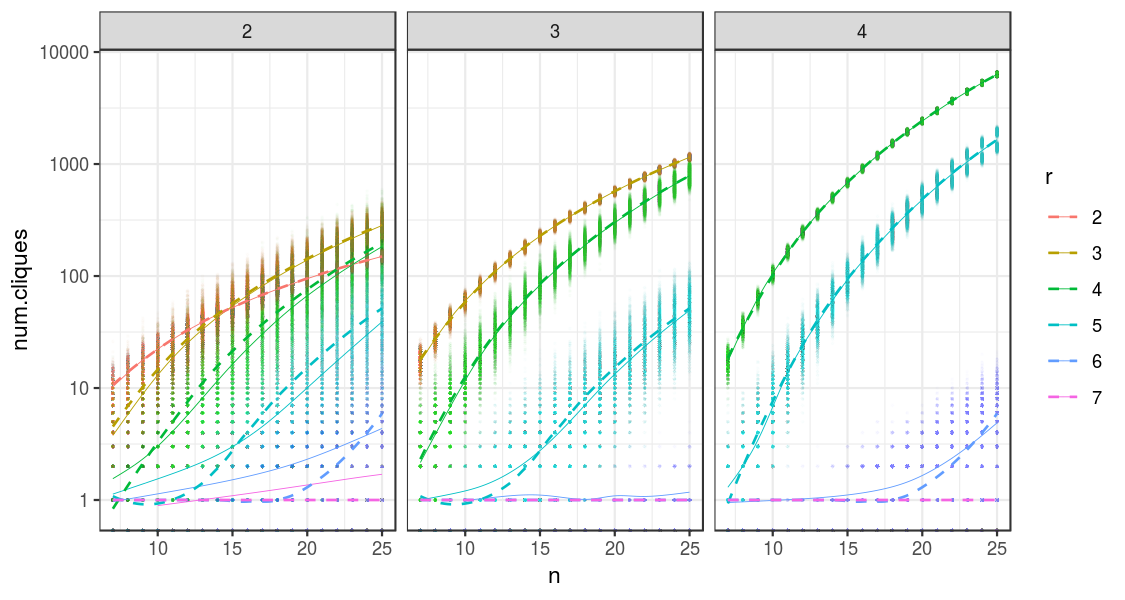
\includegraphics[width=1\textwidth]{cliqueCounter/R/numCliques.png}

We can also count the number of edges covered for different sizes
of edge:

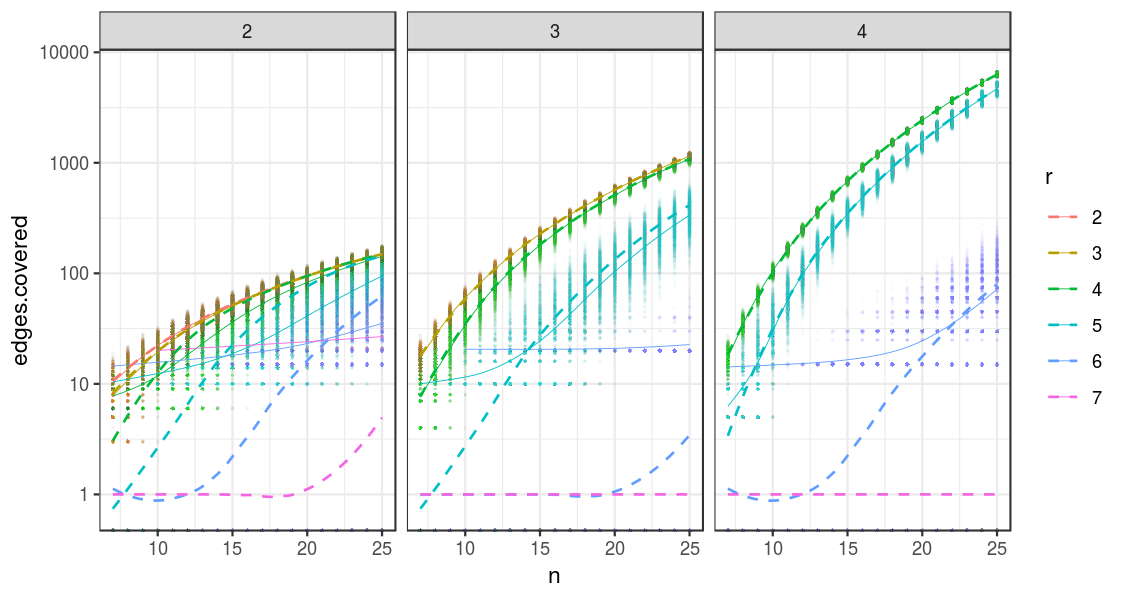
\includegraphics[width=1\textwidth]{cliqueCounter/R/edgesCovered.png}

More relevant to this problem, is the fraction of edges covered
by one of the r-cliques:

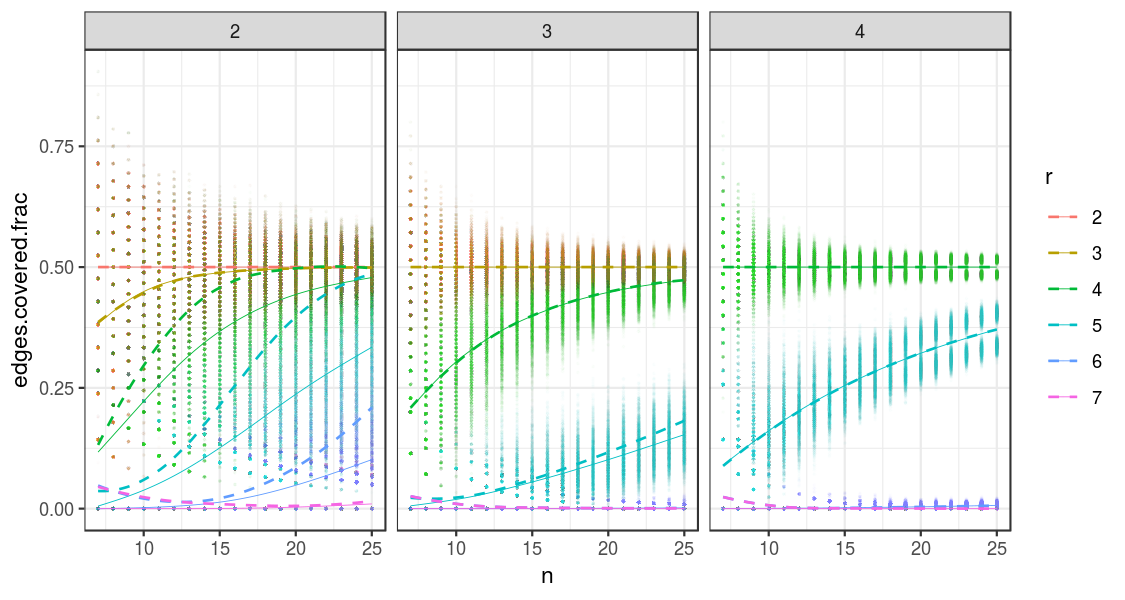
\includegraphics[width=1\textwidth]{cliqueCounter/R/fracCovered.png}

All of these
estimates appear more accurate for larger edge sizes and graphs, which
makes sense to me, because of the Central Limit Theorem.

\subsubsection{The bound implied by this covering}

We now combine the Shannon bound, together with the estimates of how many
hypercliques are needed for an average random hypergraph.
If we know the average number of gates needed to find many sets of cliques, and
can do that efficiently using a ``small'' number of clique detectors,
then we hopefully get a bound on the number of gates in each clique detector.

On the left side, we have
the Shannon bound on how many gates are needed, for an average function
chosen randomly from BUGGY-$k$-CLIQUE.

On the right side, we have
the average number of gates which suffice for us to cover the hyperedges
(which are $K_k$s in the original input graph) of an instance of
BUGGY-$k$-CLIQUE.
We will assume that we can detect $k$-cliques on $r$-vertex graphs using
$h(r)$ NAND gates, for some function $h$.
We then sum up the total cost (in NAND gates)
of covering that many $r$-vertex hypergraphs in a larger $n$-vertex graph.

\[
\underbrace{\sqrt{n \choose k} - {n \choose 2}}_\text{average number of gates needed}
\le \sum_{r=k}^n
\underbrace{h(r)}_\text{cost, in gates}
\cdot
\underbrace{{n \choose r} \cdot 2^{-{r \choose k}}}_\text{expected number of $K_r^k$s}
\cdot
\underbrace{\Big[1 - 2^{-{r \choose {k-1}}}\Big]^{n - r}}_\text{fraction of $K_r^k$s not covered by a $K_{r+1}^k$}
\]

We then hope that if we set $h$ to, say, a small enough
function, we'll get a contradiction. Note that to bound $h(r)$, we need
$n$ to be much larger (so that much of the graph is covered with $r$-vertex
hypercliques).

I tried to simplify this formula (e.g. by trying to change it into an
integral), without much luck.
However, even
without simplifying this formula more, we could computing
the number of graphs covering for a variety of
 $n$ and $k$, and solving for the minimum values of
$h(r)$ (a lower bound on the
number of gates needed) using a linear program solver.
I haven't done this so far.

\subsection{Using just one size of hyperclique} \label{oneCliqueSize}

As that expression is complicated, we seek a simpler (but
presumably weaker) bound.
As noted earlier, there is a strong incentive to use the largest
hypercliques possible, as our assumption is that this will be less
expensive. In theory, it seems useful to cover a graph with a variety
of sizes of clique.

However, we don't expect large hypercliques to be frequent.
Indeed, \cite{bollobas1993clique} covers random (non-hyper)-graphs
with cliques of just
one size.
This suggests the simpler strategy of picking one intermediate
size of hyperclique,
and only use clique-finding for that size problems. For smaller problems,
just use one NAND gate per hyperedge (clique).
This strategy
presumably is less efficient, but seems easier to analyze.

(In terms of the previous metaphor, perhaps Yoyodyne has abandoned trying to
create a custom chip for every possible hypergraph. Instead, they have
developed a CISC chip
with a CLQ instruction, which checks for a clique
of any given size. But then, a contingent of chip architects, fresh from
reading \cite{hennessy2011computer}, argue that they're better off building
a chip with a CLQ instruction which only works for a fixed size of graph.
Maybe this simplifies pipelining the clique detector...)

Suppose that we pick $r$ such that $k < r < n$; in the given hypergraph,
we will cover every $K_r^k$ with some circuit; all remaining hyperedges
(cliques) will simply be detected with one NAND gate each.
In the bound below,
the LHS is the Shannon bound on the average number
of gates.

Assume that this subcircuit, for finding $k$-cliques in an $r$-vertex graph,
requires $h(r)$ NAND gates, for some
function $h$. Then,
the cost to cover all edges in a $K_r^k$ is simply $h(r)$ times the
expected number of $K_r^k$s (as estimated in \cite{bollobas1976cliques}).
This is the second term in the RHS, below.

How many edges are left over? These are ``expensive'', as we're
paying one gate for each. How likely is an edge to be ``missed''
by the larger cliques? There are $k$ edges in the clique, so to form
the larger clique, we need to pick $r-k$ additional vertices from
the $n-k$ vertices not in the edge. Given that edge is chosen, there
are another ${r \choose k} - 1$ edges which all have to be included,
each with probability $1/2$.
This is the first term in the RHS, below.

\[
\underbrace{\sqrt{n \choose k} - {n \choose 2}}_\text{Shannon bound}
\le
\underbrace{\frac{1}{2} {n \choose r} (1 - 2^{1-{r \choose k}}) ^ {n-k \choose r-k}}
_\text{Gates for edges not covered by a clique}
   + \underbrace{h(r) \cdot {n \choose r} 2^{-{r \choose k}}}
_\text{Gates for edges covered by a clique}
\]

The nice thing about this sum is that it's only two terms (rather than
the summation above).

\subsubsection{Optimizing the bound}

We now try to see what, if anything, this bound implies. Note again
(somewhat confusingly) that in terms of the original clique-finding problem,
this is bounding the number of NAND gates needed to find $k$-cliques in an
$r$-vertex (non-hyper)-graph. We will be choosing $n$ to be some much larger
number (large enough to guarantee that many hyperedges are covered by
hypercliques).

One problem that arises is numerical: we are multiplying huge numbers
(the number of possible hypercliques) by infinitesimal numbers
(the probability of an edge being present). Initially, I used R, and
then used Julia's arbitrary-precision arithmetic.

When I attempted to optimize this for a tiny case, $k=5$ and $r=6$,
searching for $n$ up to 500,
this did eventually get above zero.
The maximum was when $n=420$, at which point the bound was
... $3.1355 \cdot 10^{-6}$.
Since there must be an integral number of NAND gates, we can then round up
to ``at least one NAND gate.''
(This is reminiscent of the ``chipmunks in trees''
problem described in \cite{ross2006first}, p. 344).
That bound is uninspiring, but that was for a tiny case, which might be
expected to be difficult to find a large lower bound for.

\subsubsection{Dealing with numerical issues}

When I tried maximizing for larger (presumably harder)
problems, I started using up my laptop's
memory (all 8 Gb of it). Also, computing the bound
was fairly slow. I assume that the
issue was that Julia's {\tt Rational} type was spending much time reducing
fractions to simplest form.

In order to work around this, I rewrote parts of the code,
approximating based on the fact that

\[
\lim_{a\to\infty} (1 - a^{-1})^{a} = e^{-1}
\]

(In fact, $e^{-1}$ is an upper bound). This implies

\[
\lim_{a\to\infty} (1 - a^{-1})^{b} = e^{-\frac{b}{a}}
\]

(Although now I'm wondering if it's a problem if $b$ is {\em also}
big).

The probability of a hyperedge not being covered by an $r$-hyperclique is

\[
p = [1 - 2 ^ {1-{r \choose k}}] ^ {n-k \choose r-k}
\]

Letting $a = 2^{{r \choose k}-1}$ and $b = {n-k \choose r-k}$, we get

\[
\log p \approx - \frac{{n-k \choose r-k}} {2^{[{r \choose k}-1]}}
\]

%% \log p \approx -\frac{n-k \choose r-k}{ 2^{({r \choose k}-1)} }




\section{Related work}

This bound relies heavily on a modification of Shannon's original
function-counting argument \cite{shannon_synthesis_1949}.

Broadly speaking, the idea of using an upper bound to prove a lower bound
is not new. Aaronson describes this as ``ironic complexity theory''
\cite{aaronson_pnp}, and mentions several recent applications of it.

Probabilistic graph theory has often been used in
lower bounds and algorithms. A well-known example is Razborov's lower
bound on the complexity of detecting cliques using monotone circuits
\cite{Razborov85lowerbounds}.

\section{Conclusion}

We first give a lower bound on finding {\em some} set of cliques.
It is a modified form of Shannon's counting argument
\cite{shannon_synthesis_1949}.

We also present a connection between this argument and the problem of covering
hypergraphs with hypercliques.
It seems that if an arbitrary hypergraph can be covered with 
``large'' hypercliques,
then this would give a lower bound on the NAND gates required to
detect cliques.

Unfortunately, using one (relatively simple) strategy for doing this covering,
the bound was, like, less than one. Possibly improving the covering
strategy would help, but I'm not convinced it would help much.

This lower-bound strategy also seems potentially
relevant to quantum computing,
as the argument makes few restrictions on the sort of gates used.
If it's the case that any function in BQP can be represented
as a circuit made of discrete quantum gates, which can be
ORed together, then clique detection isn't in BQP.
However, I'm not sure what sort of quantum gates would be
appropriate.

\section{Acknowledgements}

The author would like to thank William Gasarch for introducing him
to circuit complexity, probabilistic proofs about graphs,
and lower bound strategies.
He would also like to thank the maintainers of
several entertaining and relevant blogs: the Computational Complexity blog
(Lance Fortnow and William Gasarch), 
G\"odel's Lost Letter (Richard Lipton and Ken Regan),
and Shtetl-Optimized (Scott Aaronson). 

\bibliography{references}
\bibliographystyle{abbrv}

\end{document}

